% TODO: trust model of the project
% TODO: move Veritas def to impl? Replace with more pre-testing, using and eval of other systems that inspired/guided design of Veritas
% TODO: PCC

\chapter{Preparation}\label{ch:prep}

This chapter gives the background needed to understand the design of Veritas: the type-system machinery used to express safety properties, the related verification systems that informed the design, and the engineering decisions that fix the project's trust boundary. The aim is to establish only the theory and design context needed for the implementation that follows.

\section{Background}\label{sec:background}

\subsection{Type systems and safety}

The fundamental theorem that connects type systems to safety is \emph{type soundness}: a well-typed program cannot `go wrong' at runtime~\cite{Milner1978Theory}. Wright and Felleisen formalised this via the \emph{progress} and \emph{preservation} lemmas~\cite{Wright1994Syntactic}:

\begin{tcolorbox}[colback=gray!5!white,colframe=black!70,title=\textsc{Type soundness}]
  \textbf{Progress}

  If $\emptyset \vdash e : \tau$, then either $e$ is already a value, or there exists some expression $e'$ such that $e \to e'$.

  \medskip
  \textbf{Preservation}

  If $\emptyset \vdash e : \tau$ and $e \to e'$, then $\emptyset \vdash e' : \tau$.
\end{tcolorbox}

% \textbf{Progress.} If $\emptyset \vdash e : \tau$, then either $e$ is already a value, or there exists some expression $e'$ such that $e \to e'$.
%
% \textbf{Preservation.} If $\emptyset \vdash e : \tau$ and $e \to e'$, then $\emptyset \vdash e' : \tau$.

% \noindent Progress states that a closed well-typed program never becomes stuck before it has produced a value: whenever evaluation has not yet finished, there is always a valid next reduction step. Preservation states that evaluation does not invalidate typing: every execution step preserves the type established statically. 
\noindent Starting from a well-typed program, repeated evaluation can neither get stuck in an ill-defined intermediate state (progress) nor escape the guarantees expressed by its type (preservation). In practice, this is the formal basis for claims such as ``a well-typed array access cannot go out of bounds'' or ``a well-typed arithmetic expression is not applied to a boolean''.

% An important consequence of tractability is that type systems are \emph{sound} but not \emph{complete}: every accepted program is safe, but some safe programs will be rejected. This is a deliberate trade-off---soundness is essential for guarantees, while completeness is sacrificed for decidability. Refinement types push this boundary by encoding richer invariants, but the fundamental incompleteness remains.

The relevant distinction for Veritas is whether a type system can express facts about values, not only broad categories of values:

\begin{table}[H]
  \centering
  \small
  \begin{tabular}{p{0.24\textwidth} p{0.28\textwidth} p{0.36\textwidth}}
    \hline
    \textbf{Type system} & \textbf{Can express} & \textbf{Limitation for Veritas} \\
    \hline
    Simple types & Broad categories such as integers, booleans, and pointers & Cannot state that an index is in bounds. \\
    Hindley--Milner~\cite{Milner1978Theory} & Polymorphic types with strong inference & Still cannot express value-dependent safety facts. \\
    Refinement types & Predicates over base values & Requires SMT-backed proof obligations. \\
    Full dependent types~\cite{MARTINLOF1982153} & Arbitrary propositions as types & Often requires explicit proof terms. \\
    \hline
  \end{tabular}
  \caption{Type-system expressiveness relevant to Veritas.}
  \label{tab:type-system-spectrum}
\end{table}

\subsection{Dependent types and refinement types}\label{sec:dependent-types}

In a dependently typed language, types may depend on terms. The canonical example is the type of vectors indexed by their length, $\mathrm{Vec}(A, n)$, where $n$ is a natural number. A function that accesses the $i$-th element can require in its type that $0 \le i < n$, statically ruling out out-of-bounds accesses:
\[
  \mathrm{lookup} :
  \mathrm{Vec}(A,n) \to
  \{i\!:\!\mathtt{int} \mid 0 \le i < n\} \to A
\]
Full dependent type systems, such as those in Coq and Agda~\cite{Bove2009Agda}, can express arbitrary propositions in higher-order logic as types (via the Curry--Howard correspondence), but this generality comes at a cost: type checking is expensive and may require the programmer to construct explicit proof terms.
% TODO: coq, agda: higher-order logic
% \[
%   \mathrm{lookup} : \forall A, n.; \mathrm{Vec}(A,n) \to \mathrm{Fin}(n) \to A
% \] where Fin(n) is the type of all valid indices n

Refinement types~\cite{Rondon2008Liquid} are a practical restriction of full dependent types in which a base type is decorated with a logical predicate drawn from a decidable logic. For example, the type $\{v\!:\!\mathtt{int} \mid v > 0\}$ classifies integers that are strictly positive. Notably, subtyping between refinement types reduces to logical implication:
\begin{tcolorbox}[colback=gray!5!white,colframe=black!70,title=\textsc{Refinement subtyping}]
  \[
    \{v\!:\!\mathtt{int} \mid P(v)\}
    <:
    \{v\!:\!\mathtt{int} \mid Q(v)\}
    \quad\text{when}\quad
    P(v) \Rightarrow Q(v)
  \]
\end{tcolorbox}
% $\{v\!:\!\mathtt{int} \mid P(v)\} <: \{v\!:\!\mathtt{int} \mid Q(v)\}$ holds when $P(v) \Rightarrow Q(v)$ is valid. 
Because the predicates are drawn from a decidable theory (typically quantifier-free linear arithmetic), this implication check can be delegated to an SMT solver.

A particularly useful special case is the singleton type, written $\mathtt{int}(n)$, which is inhabited by exactly the integer $n$. Singleton types arise naturally from Xi and Pfenning's work on Dependent ML~\cite{Xi1999DML}, where integer index expressions are used to track array sizes and loop bounds. Singleton types can propagate exact values through arithmetic:
\[
  \begin{array}{rcl}
    x &:& \mathtt{int}(3) \\
    y &:& \mathtt{int}(5) \\
    x + y &:& \mathtt{int}(8)
  \end{array}
\]
% if $x : \mathtt{int}(3)$ and $y : \mathtt{int}(5)$, then $x + y : \mathtt{int}(8)$. 
This enables compile-time verification of array bounds when indices are statically known.

% TODO: [because of advantages] Veritas' type system extends a simple base type system (integers, booleans, arrays) with refinement types to encode value-dependent invariants.

\subsection{Bidirectional type checking}

Bidirectional type checking~\cite{Pierce2000Local} structures type checking into two mutually recursive judgements:

\begin{tcolorbox}[colback=gray!5!white,colframe=black!70,title=\textsc{Bidirectional judgements}]
  \paragraph{Type checking} verifies that expression $e$ has expected type $\tau$: $\Gamma \vdash e \leftarrow \tau$. \\

  \paragraph{Type synthesis} infers a type $\tau$ for expression $e$: $\Gamma \vdash e \Rightarrow \tau$.
\end{tcolorbox}
% \begin{itemize}
%   \item \emph{Type checking} takes a context $\Gamma$, program $e$ and type $\tau$ as input and produces a true/false output reflecting whether $e$ is well-typed: $\Gamma \vdash e \leftarrow \tau$
%   \item \emph{Type synthesis} takes a context $\Gamma$ and program $e$ as input and produces a types $\tau$ as output: $\Gamma \vdash e \Rightarrow \tau$
% \end{itemize}

\noindent The two modes are connected by a subsumption rule:
$$
  \frac{\Gamma \vdash e \Rightarrow \sigma \quad \sigma <: \tau}{\Gamma \vdash e \leftarrow \tau}
$$
% \noindent To check an expression against a type $\tau$, one may synthesise a type $\sigma$ and then verify $\sigma$ is a subtype of $\tau$.

% type synthesis ($\Gamma \vdash e \Rightarrow \tau$), which infers the type of an expression bottom-up, and type checking ($\Gamma \vdash e \Leftarrow \tau$), which verifies that an expression has a given type top-down. The two modes are connected by a subsumption rule; to check an expression against a type $\tau$, one may synthesise a type $\sigma$ and then verify $\sigma <: \tau$.

% Alternative approaches have significant drawbacks. Full type inference in the style of Hindley--Milner requires unification, which does not extend naturally to subtyping or refinement types; the lattice structure of refinement types means there is no unique principal type for many expressions. At the other extreme, requiring complete type annotations on every expression is impractical. Bidirectional checking offers a middle ground where the programmer annotates introduction forms (function signatures, let-bindings) and the system infers the rest.

For refinement types, synthesis can produce precise local facts---integer literals synthesise singleton types, and arithmetic synthesises refinements relating the result to its operands. Checking then verifies subtyping against the expected type. In Veritas, programmers annotate function boundaries and mutable declarations; intermediate refinements are inferred.

In Veritas, the bidirectional structure also threads the typing context through the judgements. Both synthesis and checking accept a context and return an updated context, reflecting changes from mutable variable assignments and newly learned refinement propositions.

\subsection{SMT-based verification}
\label{sec:smt-based-ver}
% TODO: diagram of SMT-solver with formulae

Satisfiability Modulo Theories (SMT) extends boolean satisfiability to richer logics. The theories relevant to Veritas are linear integer arithmetic, arrays, and uninterpreted functions. Z3~\cite{DeMoura2008Z3} is used because it is mature, widely deployed, and already used in systems that influenced Veritas, including Liquid Haskell, Dafny, and F*.

The technique for using an SMT solver as a refinement type checker is \textit{proof by refutation}~\cite{Rondon2008Liquid}. To check whether $\phi \vdash P$ holds, Veritas checks whether $\phi \wedge \lnot P$ is unsatisfiable:

\begin{tcolorbox}[colback=gray!5!white,colframe=black!70,title=\textsc{SMT proof obligation}]
\begin{verbatim}
assume all propositions in phi
assert not P
accept the obligation iff Z3 returns UNSAT
\end{verbatim}
\end{tcolorbox}

If the solver returns \textsc{unsat}, then $P$ must hold under $\phi$; if it returns \textsc{sat}, the countermodel witnesses a failed proof obligation.

This approach means that the \textit{discharge} of proof obligations is fully automatic: the programmer never constructs proof terms. However, the programmer must still supply the specifications from which these obligations arise---type annotations, function contracts, and loop invariants. The automation lies in checking, not in specification.
% TODO: state that annotations are not a burden, but guidance, minimise programmer error, clarifies logic/control flow?

In Veritas, the SMT solver is invoked at several points: subtyping checks between refinement types (where the solver verifies that one predicate implies another), array bounds verification (where the solver must prove that an index lies within $[0, N)$), and function contract verification (where preconditions and postconditions are checked at call sites and return points respectively).

% For quantified specifications such as $\forall i \in [0, n).\; \mathit{arr}[i] \ge 0$, the translation uses Z3's built-in quantifier support: $\forall i.\; (0 \le i \wedge i < n) \Rightarrow \mathit{arr}[i] \ge 0$, where the array is represented as a Z3 array sort. Existential quantifiers are handled dually, asserting $\exists i.\; (a \le i \wedge i < b) \wedge P$. While quantified formulae move outside the decidable fragment of LIA, Z3's E-matching and model-based quantifier instantiation heuristics handle the bounded quantifiers that arise in practice effectively.

\subsection{Type-preserving compilation}\label{sec:type-pres-background}

Conventional compilers erase types after type checking, discarding the safety guarantees established by the type system. The generated machine code is subsequently trusted on the basis that the compiler is correct, an assumption that is difficult to verify for large, complex compilers. Type-preserving compilation~\cite{Morrisett1999SystemF} retains type information through every intermediate representation in the pipeline. This enables the property that the compiled output can be independently verified without trusting the compiler. If a bug in the compiler produces type-incorrect code, the type annotations on the output will be inconsistent, and the verifier will reject it.
% TODO: give examples of what attacks from an adversarial compiler can be detected

\subsection{Proof-carrying code}\label{sec:pcc-background}

The idea of shipping machine code together with a checkable proof of its safety was formalised by Necula as proof-carrying code (PCC)~\cite{Necula1997PCC}. In PCC, the code producer (i.e., compiler) generates both executable code and a safety proof; the code consumer (e.g., an operating system loader) checks the proof against a safety policy before executing the code. The proof checker is small and can be verified more quickly and easily than the entire compiler. Type-preserving compilation can be seen as a particular instance of PCC where the `proof' takes the form of type annotations.

\subsection{Dependently Typed Assembly}\label{sec:dtal-background}

Xi and Harper introduced DTAL as a target for type-preserving compilation from DML~\cite{Xi1999DML} and Xanadu~\cite{Xi2000Xanadu}. DTAL augments assembly with two key forms of type annotation:
\begin{itemize}
  \item \textbf{Label signatures}: each basic block entry point is annotated with existentially quantified index variables and the types expected for each register on entry, enabling modular, block-by-block verification.
  \item \textbf{Register types}: types may depend on index variables, so that a register's type tracks its exact value (e.g., $\mathtt{int}(i)$) or the size of an array it points to (e.g., $\mathtt{int\;array}(n)$).
\end{itemize}

\noindent A DTAL loop header binds index variables and declares register types in terms of them:

\begin{verbatim}
  loop:  {m:nat, n:nat | m <= n, i:nat}
         [r1: int array(m), r2: int array(n), r3: int(m), r4: int(i)]
         sub   r5, r4, r3       // r5 <- i - m
         bgte  r5, finish       // if i >= m, exit
         load  r5, r1(r4)       // safe: i < m
         store r2(r4), r5       // safe: i < n (since m <= n)
         add   r4, r4, 1
         jmp   loop
\end{verbatim}

\noindent The branch \texttt{bgte r5, finish} refines the type state: on the fall-through path, the type system knows $i < m$, which makes the subsequent \texttt{load} and \texttt{store} provably safe without any runtime bounds check. Xi and Harper proved that well-typed DTAL programs cannot violate the constraints of the type system.

Veritas implements its own DTAL variant based on Xi and Harper's design, extended to support the Veritas refinement type system and targeting x86-64. The compiler translates the source language through a typed intermediate representation (TIR) to DTAL, preserving refinement types at each stage, and finally emits x86-64 machine code as an ELF executable. Hereafter, `DTAL' refers to this Veritas-specific variant unless otherwise noted; the original is referred to as `Xi and Harper's DTAL'.

\section{Related work and design influences}
\label{sec:related-work}
% TODO: include diagram

Veritas combines automated refinement checking, systems-language design, and proof-carrying code. The systems below matter because each fixes a different point in the design space: automation, expressiveness, systems orientation, or low-level trust.

\subsection{Refinement types and automated verification}
Liquid Haskell~\cite{Vazou2014Refinement} and Liquid Types~\cite{Rondon2008Liquid} provide the main precedent for SMT-backed refinement checking. Dafny~\cite{Leino2010Dafny} similarly uses SMT solving for imperative contracts and loop invariants. Veritas borrows this style of automatic proof discharge, but preserves the resulting constraints down to assembly rather than erasing them after source-level verification.

\subsection{Foundational and dependent verification}
F*~\cite{Swamy2016Dependent} and RefinedC~\cite{Sammler2021RefinedC} offer stronger theoretical foundations through dependent types or separation logic. RefinedC, for example, produces machine-checked Coq proofs for existing C code. Veritas deliberately accepts a weaker foundation---SMT-backed checking rather than foundational proof---to keep proof obligations automatic once specifications are supplied.

\subsection{Verifiable systems languages}
ATS (Applied Type System)~\cite{Xi2003Applied} is the closest predecessor in spirit: it targets systems programming with dependent types and zero runtime overhead. The key difference is architectural. ATS proves properties at compile time and then emits C, leaving the ATS and C compilers in the TCB. Veritas instead preserves types into DTAL so that the low-level target can be checked independently.

Figure~\ref{fig:verification-landscape} summarises the trade-off between expressiveness and automation across the systems discussed above.

\begin{figure}[H]
  \centering
  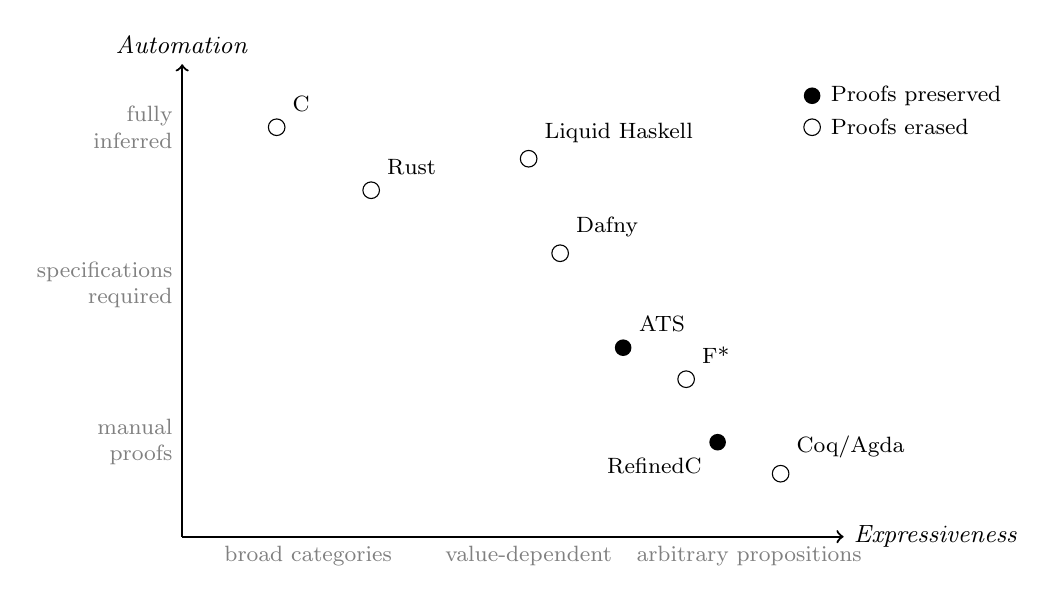
\begin{tikzpicture}[
      every node/.style={font=\small},
      filled/.style={circle, fill=black, inner sep=0pt, minimum size=6pt},
      hollow/.style={circle, draw=black, fill=white, inner sep=0pt, minimum size=6pt},scale=0.8
    ]
    % Axes
    \draw[->, thick] (0,0) -- (10.5,0) node[right] {\textit{Expressiveness}};
    \draw[->, thick] (0,0) -- (0,7.5) node[above] {\textit{Automation}};

    % Axis labels
    \node[below left, font=\footnotesize] at (0,0) {};
    \node[below, font=\footnotesize, text=gray] at (2,0) {broad categories};
    \node[below, font=\footnotesize, text=gray] at (5.5,0) {value-dependent};
    \node[below, font=\footnotesize, text=gray] at (9,0) {arbitrary propositions};
    \node[left, font=\footnotesize, text=gray, align=right] at (0,1.5) {manual\\proofs};
    \node[left, font=\footnotesize, text=gray, align=right] at (0,4) {specifications\\required};
    \node[left, font=\footnotesize, text=gray, align=right] at (0,6.5) {fully\\inferred};

    % Systems (hollow = proofs erased, filled = proofs preserved)
    % C: low expressiveness, high automation (no proofs needed, but no safety)
    \node[hollow, label={[font=\footnotesize]above right:C}] at (1.5,6.5) {};

    % Rust: moderate expressiveness (ownership), high automation
    \node[hollow, label={[font=\footnotesize]above right:Rust}] at (3,5.5) {};

    % Liquid Haskell: good expressiveness, high automation (predicate inference)
    \node[hollow, label={[font=\footnotesize]above right:Liquid Haskell}] at (5.5,6) {};

    % Dafny: good expressiveness, moderate automation (requires contracts/invariants)
    \node[hollow, label={[font=\footnotesize]above right:Dafny}] at (6,4.5) {};

    % Veritas: similar expressiveness to Dafny, slightly less automated, proofs preserved
    % \node[filled, label={[font=\small\bfseries]below left:Veritas}] at (5.5,4) {};

    % ATS: high expressiveness, lower automation (manual proofs sometimes needed), proofs preserved at compile time
    \node[filled, label={[font=\footnotesize]above right:ATS}] at (7,3) {};

    % F*: very expressive, moderate-low automation
    \node[hollow, label={[font=\footnotesize]above right:F*}] at (8,2.5) {};

    % RefinedC: very expressive, low automation (Coq proofs), proofs preserved
    \node[filled, label={[font=\footnotesize]below left:RefinedC}] at (8.5,1.5) {};

    % Coq/Agda: most expressive, lowest automation
    \node[hollow, label={[font=\footnotesize]above right:Coq/Agda}] at (9.5,1) {};

    % Legend
    \node[filled, label={[font=\footnotesize]right:Proofs preserved}] at (10,7) {};
    \node[hollow, label={[font=\footnotesize]right:Proofs erased}] at (10,6.5) {};

  \end{tikzpicture}
  \caption{Verification systems positioned by expressiveness of their type/specification language and degree of automation.\centering}
  \label{fig:verification-landscape}
\end{figure}

% \subsection{Feature Comparison}
%
% Table~\ref{tab:comparison} summarises how Veritas compares to these related tools across five key dimensions. The distinguishing feature of this project is the combination of SMT-backed refinement types with type-preserving compilation, culminating in a dependently typed assembly language that supports completely independent verification.
%
% \begin{table}[h]
% \centering
% \begin{tabular}{l c c c c c}
% \hline
%  & \textbf{Refinement} & \textbf{SMT-} & \textbf{Systems} & \textbf{Type-preserving} & \textbf{Independent} \\
%  & \textbf{types} & \textbf{backed} & \textbf{language} & \textbf{compilation} & \textbf{verifier} \\
% \hline
% Liquid Haskell & \checkmark & \checkmark & & & \\
% Dafny & \checkmark & \checkmark & \checkmark\textsuperscript{$\dagger$} & & \\
% F* & \checkmark & \checkmark & & & \\
% ATS & \checkmark & & \checkmark & & \\
% RefinedC & \checkmark & & \checkmark & & \checkmark\textsuperscript{*} \\
% \textbf{Veritas} & \checkmark & \checkmark & \checkmark & \checkmark & \checkmark \\
% \hline
% \end{tabular}
% \caption{Feature comparison of verification systems. (\textsuperscript{*}RefinedC produces Coq proofs rather than a standalone verifier. \textsuperscript{$\dagger$}Dafny can compile to imperative targets but is not strictly a low-level systems language.)}
% \label{tab:comparison}
% \end{table}

\section{Design decisions}\label{sec:design-decisions}

The central design task was to realise the trust architecture without making the source language unusable or the trusted backend too large.

\subsection{Compiler architecture}

A central architectural decision is that the compiler is \textit{untrusted}. Rather than proving the compiler correct, Veritas relies on a standalone verifier that re-checks the compiler's low-level output. Compiler bugs should therefore cause rejection, not unsafely accepted code. Figure~\ref{fig:trust-pipeline} shows the resulting boundary: type information flows through the compiler, but trust begins only at the verifier and direct encoder.

\subsection{Trust model and TCB reduction}

The implementation was structured to move the verification boundary progressively lower in the pipeline:

\begin{enumerate}
  \item \textbf{Virtual DTAL verification}: the verifier checks DTAL with virtual registers. The TCB includes the verifier, Z3, register allocation, instruction selection, and the x86-64 encoder.
  \item \textbf{Physical DTAL verification}: the verifier checks DTAL \textit{after} register allocation. Register allocation and instruction selection are removed from the TCB. The TCB is now the verifier, Z3, and a trivial direct encoder.
  \item \textbf{Runtime and bare-metal}: the runtime is kept small enough to audit by inspection, and a bare-metal target removes the OS from the TCB entirely.
\end{enumerate}

\begin{figure}[ht]
  \centering
  \begin{tikzpicture}[
      scale=0.85,
      transform shape,
      node distance=0.9cm and 1.1cm,
      box/.style={draw, rounded corners, minimum height=1.0cm, minimum width=4.0cm, align=center, font=\small},
      typed/.style={box, fill=blue!10},
      untyped/.style={box, fill=gray!10},
      trusted/.style={box, fill=green!12},
      arrow/.style={-Latex, thick}
    ]
    \node[untyped] (src) {Source\\\texttt{.veri}};
    \node[typed, right=of src] (tast) {Typed AST};
    \node[typed, right=of tast] (tir) {Typed SSA\\(TIR)};
    \node[typed, right=of tir] (dtal) {DTAL};

    \node[typed, below=1.6cm of dtal] (phys) {Physical DTAL};
    \node[trusted, left=of phys] (ver) {Independent Verifier};
    \node[trusted, left=of ver] (enc) {Direct Encoder};
    \node[untyped, left=of enc] (elf) {ELF / Machine Code};

    \draw[arrow] (src) -- (tast);
    \draw[arrow] (tast) -- (tir);
    \draw[arrow] (tir) -- (dtal);
    \draw[arrow] (dtal) -- node[right=0.35cm, font=\scriptsize, align=left, fill=white, inner sep=1pt] {physalloc\\(untrusted)} (phys);
    \draw[arrow] (phys) -- (ver);
    \draw[arrow] (ver) -- (enc);
    \draw[arrow] (enc) -- (elf);

    \draw[dashed, rounded corners]
    ([xshift=-0.35cm,yshift=0.35cm]tast.north west) --
    ([xshift=0.35cm,yshift=0.35cm]dtal.north east) --
    ([xshift=0.35cm,yshift=-0.35cm]dtal.south east) --
    ([xshift=0.35cm,yshift=-0.35cm]phys.south east) --
    ([xshift=-0.35cm,yshift=-0.35cm]phys.south west) --
    ([xshift=-0.35cm,yshift=-0.35cm]dtal.south west) --
    ([xshift=-0.35cm,yshift=-0.35cm]tast.south west) --
    ([xshift=-0.35cm,yshift=0.35cm]tast.north west);
    \node[font=\small, above] at ([yshift=0.35cm]tir.north) {untrusted compiler};
    \node[draw, dashed, rounded corners, fit=(ver)(enc), inner sep=0.25cm,
      label={[font=\small]below:trusted core}] {};
  \end{tikzpicture}
  \caption{Veritas compilation pipeline and trust boundary.}
  \label{fig:trust-pipeline}
\end{figure}

\subsection{Source language design}

Veritas is a small imperative language with C-like syntax, inspired by Xi and Harper's Xanadu. It supports integers, booleans, fixed-size arrays, mutable and immutable variables, loops, and functions. The type system adds singleton types, refinement types, contracts, bounded quantifiers, and loop invariants.

The key expressiveness choice was bounded quantification. Scalar refinements can prove facts about individual values, but algorithms such as binary search need array-wide properties such as sortedness. A precondition such as $\mathbf{forall}\ i\ \mathbf{in}\ 0..n\ \{\ \mathit{arr}[i] \le \mathit{arr}[i + 1]\ \}$ expresses such properties while keeping verification close to SMT-friendly fragments.

\subsection{DTAL target language design}

The target language is a variant of Xi and Harper's DTAL~\cite{Xi2001DTAL}, extended for Veritas refinements and x86-64. The core instruction set is deliberately RISC-like: simple instructions are easier to type, verify, and map from the SSA-style intermediate representation. DTAL then adds register type annotations, embedded constraint assertions, and declared type states at basic block entries.

I also defined DTAL with its own \textit{physical register model} (registers \texttt{r0}--\texttt{r12}, \texttt{sp}, \texttt{fp}, \texttt{lr}) that maps directly to x86-64 registers. This allows verification to occur \textit{after} register allocation: the register allocator is untrusted, and its output is verified before the final (trivial) encoding to x86-64.

\subsection{Machine code encoding and ELF generation}
% The final stages of the compilation pipeline translates verified physical DTAL to x86-64 machine code and packages it as a freestanding ELF binary. 
Rather than emitting assembly text and invoking NASM or GAS, Veritas encodes x86-64 instructions directly as bytes. This keeps an external assembler out of the TCB. The trusted path below physical DTAL is intentionally small: a one-to-one instruction mapping, a byte encoder, and an ELF generator.

The choice of x86-64 was pragmatic: it enabled direct execution and testing on the development machine. A different ISA would require replacing the instruction mapping, byte encoder, and register definitions, while leaving the DTAL type system and verifier structure largely unchanged.

\subsection{Design challenges}\label{sec:design-challenges}

Four design challenges shaped the implementation:

\paragraph{Mutable variables and refinement types.} Refinement type systems such as Liquid Haskell operate over immutable bindings, where a variable's type is fixed at its definition. Supporting mutation introduces a soundness hazard: after \texttt{x = e}, any refinement mentioning \texttt{x} may be invalidated. The solution adopted---\textit{master types}---required designing the mutable context $\Delta$ to track both a current (refinable) type and a fixed master type, with a subtyping check on every assignment.

\paragraph{Verification after register allocation.} In an initial phase of the implementation, the system verified DTAL with virtual registers and then trusted the x86-64 lowering ($\sim$1,100 lines of register allocation, instruction selection, and encoding). This placed a large, error-prone component inside the TCB. Redesigning the pipeline to verify \textit{after} register allocation required defining a physical DTAL register model, splitting the monolithic lowering into an untrusted physical allocation pass and a trivial direct encoder, and extending the verifier to handle physical instructions (prologues, spills, division expansion). This reduced the trusted backend code to $\sim$300 lines.

\paragraph{Type preservation across SSA join points.} At phi nodes in the SSA intermediate representation, two singleton types from different branches (e.g., $\mathtt{int}(3)$ and $\mathtt{int}(7)$) must be joined. The naive approach---widening to the base type $\mathtt{int}$---loses all refinement information, making downstream bounds proofs impossible. The solution was to attach \textit{existential constraints} to phi nodes, encoding that the value satisfies a constraint without fixing it to a concrete value. This mechanism was not part of Xi and Harper's original DTAL design and required extending both the TIR and the verifier.

\paragraph{SMT encoding of array properties.} Verifying array-manipulating programs requires reasoning about array contents, which involves quantified formulae. These fall outside the decidable quantifier-free fragment of linear integer arithmetic. The design restricted quantifiers to \textit{bounded} forms ($\mathbf{forall}\ x\ \mathbf{in}\ a..b$), which Z3's E-matching heuristics handle reliably in practice, at the cost of excluding unbounded quantification. This trade-off was accepted to maintain the automatability of verification.

\section{Requirements analysis}\label{sec:requirements-anal}

The requirements were categorised using the MoSCoW method to keep the project focused on type-preserving compilation and independent low-level verification.

\begin{table}[H]
  \centering
  \small
  \begin{tabular}{p{0.16\textwidth} p{0.76\textwidth}}
    \hline
    \textbf{Priority} & \textbf{Requirements} \\
    \hline
    Must-have & A high-level systems language with variables, control flow, functions, and arrays; a dependent type system with refinement and singleton types; a bidirectional type checker that delegates proof obligations to an SMT solver; a DTAL target with type states and constraint assertions; a compiler backend that preserves type information; and a standalone DTAL verifier that checks generated assembly without access to the source. \\
    Should-have & End-to-end executable generation to native x86-64 ELF binaries; advanced function contracts, including postconditions and quantified specifications; and automated tests for both safe programs and targeted rejection of unsafe programs. \\
    Could-have & Backend optimisations over the typed intermediate representation; extended language semantics such as structs, generics, and a full ownership model; and an interpreter for executing DTAL programs directly. \\
    Won't-have & A foundational, machine-checked proof of compiler correctness, since the compiler is deliberately untrusted; verification of concurrency properties; and verification of information-flow or cryptographic properties. \\
    \hline
  \end{tabular}
  \caption{MoSCoW requirements used to keep the project focused on type-preserving compilation and independent low-level verification.}
  \label{tab:moscow-requirements}
\end{table}

% \section{Evaluation plan}
%
% The evaluation aims to assess three dimensions: \textit{correctness}, \textit{overhead} (what is the cost of verification?), and \textit{expressiveness} (what can the type system express, and how large is the trusted computing base?).
%
% Correctness will be tested via suites of positive programs (expected to compile, verify, and execute correctly) and negative programs (expected to be rejected with specific errors). Verifier agreement---whether the independent DTAL verifier accepts every program the compiler produces---will serve as a cross-check of the trust architecture.
%
% Overhead will be measured quantitatively using the following metrics:
%
% \begin{itemize}
%   \item Compilation and verification time (with and without verification enabled)
%   \item SMT query count and cumulative solver time (frontend and verifier)
%   \item Output binary size compared to equivalent C programs compiled with GCC
%   \item Runtime execution time compared to C equivalents
% \end{itemize}
%
% Compilation timings will be collected using built-in instrumentation (the \texttt{--bench} flag emits per-stage JSON). Runtime benchmarking will use \texttt{hyperfine} for statistical rigour. A benchmarking harness will automate data collection across the test suite.
%
% Expressiveness will be assessed qualitatively: whether non-trivial algorithms can be verified, the annotation burden relative to executable code, and the proportion of the codebase within the trusted computing base.
%
% The language and its performance will also be compared against the existing verification systems surveyed in Section~\ref{sec:related-work}. Language comparisons will examine equivalent programs across systems (where possible), considering syntax verbosity, annotation requirements, and the kinds of properties each system can express. Performance comparisons will draw on published overhead figures from Liquid Haskell, Dafny, and similar tools to contextualise Veritas's verification cost.

\section{Software engineering methodology}
\label{sec:software-eng-methodology}

\subsection{Methodology}

\paragraph{Development process.} The implementation followed an incremental pipeline-first strategy. I first built an end-to-end compiler for integer arithmetic, then extended the same path with arrays, mutation, refinements, contracts, and quantifiers. Each feature was accompanied by positive tests that should compile and negative tests that should be rejected with a specific error.

\paragraph{Version control.} Version control was managed using Git, with short-lived feature branches merged into the main branch. A GitHub Actions CI pipeline ran on each push.

\paragraph{Code quality and testing.} CI enforced \texttt{cargo fmt} and \texttt{cargo clippy}, validated example programs, and ran the test suite on Ubuntu Linux and macOS. This gave coverage across the main development platforms and different Z3/libc environments.
% TODO: unit/integration tests


\subsection{Tools and Technologies}
The project was implemented in Rust, chosen for its type system, pattern matching, and memory safety without garbage collection. Rust's ownership model also influenced the later borrow-oriented parts of Veritas.

The frontend type checker and DTAL verifier use Z3 via the \texttt{z3} Rust crate. Z3 forms part of the TCB, so maturity and wide deployment matter. It also supports the theories Veritas needs: quantifier-free LIA for refinement subtyping and bounded quantifiers for array specifications.

The \texttt{im} crate provides persistent data structures for typing contexts, enabling efficient cloning at control-flow branches.



\section{Starting point}\label{sec:starting-point}

I began with introductory knowledge of dependent type theory and verification languages, and was introduced to refinement types through Xi and Harper's DTAL. No external compiler or verifier code was used. The main new areas were Rust, SMT-backed type checking, Z3 theories, x86-64 encoding, bidirectional type checking, and the Xi et al. papers on DML, Xanadu, and DTAL.
